\chapter{龙芯 3A 处理器概述}

龙芯处理器包括三个并行发展的系列。龙芯~1 号系列处理器
主要面向嵌入式应用,龙芯~2 号超标量处理器系列主要面向桌面应用,而龙芯~3
号多核处理器系列主要面向服务器和高性能机应用。根据需要,部分龙芯~2
号可以会面向高端嵌入式应用, 部分低端龙芯~3 号处理器也可以用于高性能桌面应用。

下面,将分别对龙芯~3 号处理器系列的互联架构,及 3A 处理器的具体实现作简单的介绍。

\section{龙芯 3 号处理器系列互联架构}

龙芯 3 号处理器系列采用了可伸缩的互联结构,如图~\ref{fig:gs3-connection} 所示。
这种可伸缩构架包含了两种不同层面的互联结构:(1)片内互联,和(2)片间互联。它们都是
通过二维网格的形式实现的。图~\ref{fig:gs3-connection}(a)显示的是单个结点片内互联的情形:
一个 $8\times8$ 的交叉开关将四个处理器核及四个二级 Cache
模块连接到一起,而东(E)南(N) 西(W)北(N)四个方向可以用于与其他
结点或外设互连。 图~\ref{fig:gs3-connection}(b)和(c)则是片间互联的
示例:(b)显示了一个 $2\times 2$ 的网格连接了四个结点,即总共 16 个
处理器核;(c)则是一个 $4\times 4$ 网格连接 64 个处理器核的示意图。

\begin{figure}[htpb]
  \centering
  \begin{tabular}{ccc}
    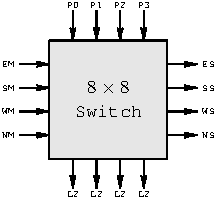
\includegraphics[scale=1.3]{gs3a-node-simple} &
    \raisebox{1cm}{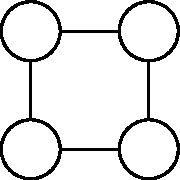
\includegraphics[scale=.65]{2x2}} &
    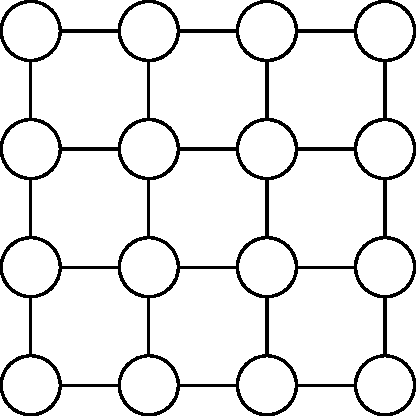
\includegraphics[scale=.65]{4x4} \\
  (a)结点结构 & (b)$2\times2$ 结点网格 & (c)$4\times4$ 结点网格
  \end{tabular}
  \caption{龙芯 3 号处理器系列互联架构}
  \label{fig:gs3-connection}
\end{figure}

图~\ref{fig:gs3-node} 给出了一个更详细的龙芯 3 号系列的结点结构图。每个结点内通过两级 AXI
交叉开关将处理器核、 二级 Cache、 内存控制器以及 IO 控制器连接在一起。 其中第一级 AXI 交叉开关 
(X1 Switch,简称 X1)连接处理器核和二级 Cache, 而第二级交叉开关(X2 Switch,简称 X2)
则连接二级 Cache 和内存控制器及其他外设。

\begin{figure}[htpb]
  \centering
  \setlength\fboxsep{15pt}
  \setlength\fboxrule{.5pt}
  \fbox{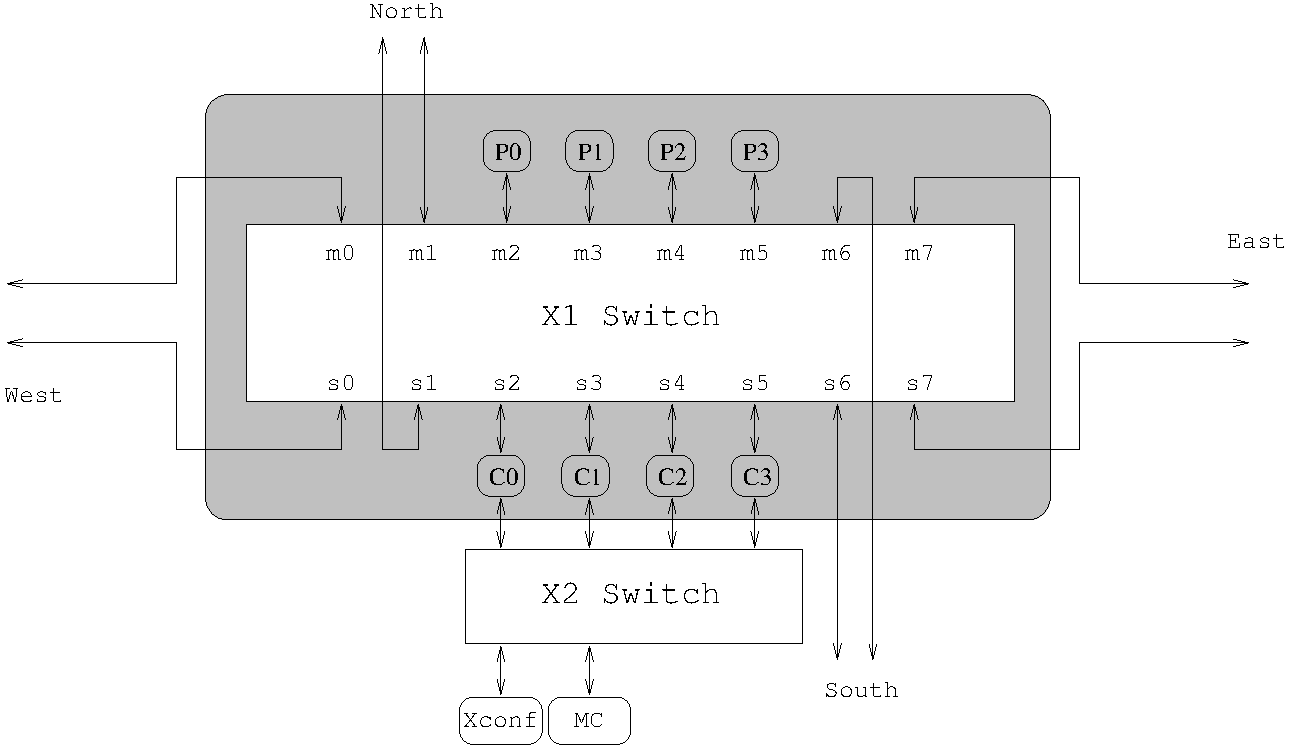
\includegraphics[scale=.7]{gs3-node}}
  \caption{龙芯 3 号节点结构}
  \label{fig:gs3-node}
\end{figure}

在每个结点中,$8\times8$ 的 X1 交叉开关通过四个主端口连接四个 GS464
处理器核(图中 P0、P1、P2、P3),四个从端口连接统一编址的四个
二级 Cache 块(图中 S0、S1、S2、S3)。 另外的四对主从端口连接东、 南、
西、北四个方向的其他结点或 I/O 外设(图中的 EM/ES、SM/SS、 WM/WS、NM/NS)。
X2 交叉开关通过四个主端口连接四个二级 Cache,至少一个从端
口连接一个内存控制器,至少一个从端口连接一个交叉开关的配置模块
(Xconf)用于配置本结点的 X1 和 X2 交叉开关的地址窗口等,还可以根据需要连接更多
的内存控制器和 IO 端口等。

龙芯 3 号系列的互连系统只是定义上层协议,而未对传输协议的实现做任何具体规
定,因此,结点之间的互连即可以采用片上网络进行实现,也可以通过 I/O 控制
链路实现多芯片的互连。以一个 4 结点 16 核系统为例,它既可以通过 4 片 4 核芯
片组成,也可以通过 2 片 8 核芯片,或基于一个单芯片 4 节点 16 核芯片组成。
由于互连系统的物理实现对软件透明, 不同配置的系统可以在相同的操作系统上运行。

\section{龙芯 3A 处理器}

龙芯 3A 是第一款龙芯 3 号多核处理器系列的处理器。 它基于可伸缩的龙芯 3
号系列多核互连架构设计, 在单个芯片上集成四个 GS464 处理器核以及四个二级 Cache
模块,并通过高速 I/O 接口实现多芯片的互连以组成更大规模的系统。

\subsection{GS464 处理器核}

GS464 是一款四发射的 64 位高性能处理器核。
该处理器核既可以作为单核处理器面向高端嵌入式应用和桌面应用,
也可以作为基本的处理器核模块用于构成片内多核系统面向服务器和高性能
机应用。图~\ref{fig:gs464-arch} 给出了 GS464 的结构示意图。
\begin{figure}[htbp]
  \centering
  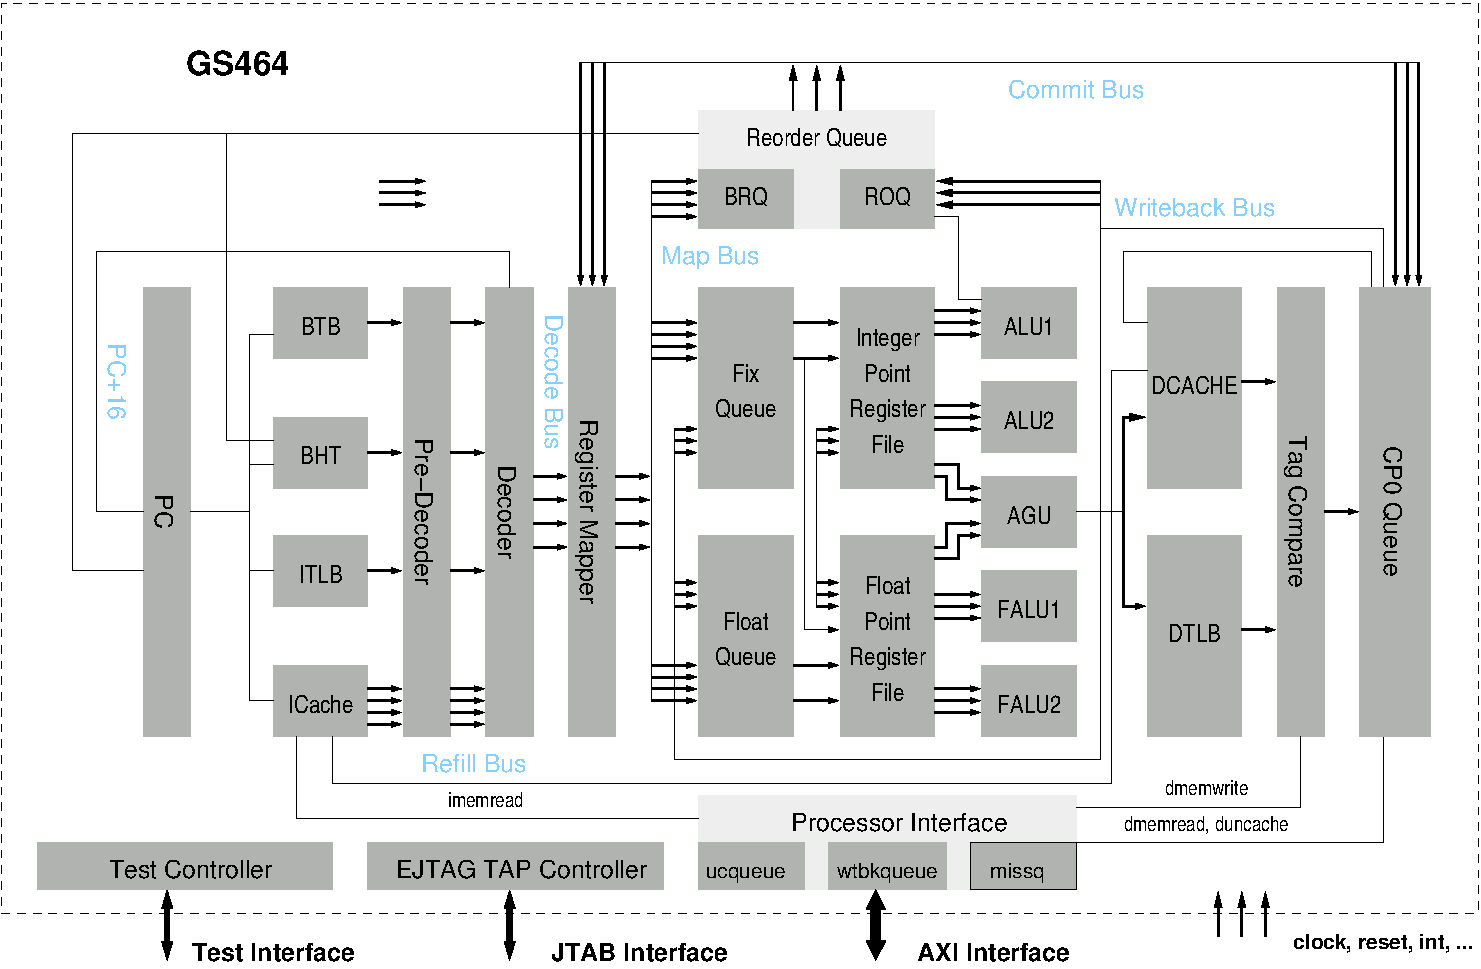
\includegraphics[scale=.55]{GS464}
  \caption{GS464 处理器核结构示意图}
  \label{fig:gs464-arch}
\end{figure}
GS464 处理器核的主要特点有:
\begin{itemize}
 \item MIPS64 兼容,并增加了 SIMD 型多媒体指令以及 x86 虚拟机指令;
 \item 四发射超标量结构:两个定点,两个浮点,和一个访存部件;
 \item 每个浮点部件都支持全流水的双精度(64 位)和单精度对(paired
   single)浮点乘加运算;
 \item 访存部件支持 128 位存储访问,支持 48 位物理地址;
 \item 支持寄存器重命名、动态调度、转移预测等乱序执行技术;
 \item 64 项全相联 TLB,独立的 16 项指令 TLB,可变页大小;
 \item 4 路组相联的一级指令 Cache 和数据 Cache, 大小各为 64KB;
 \item 支持 Non-blocking 访问及 Load-Speculation 等访存优化技术;
 \item 支持核间 Cache 一致性协议,用于片内多核处理器互联;
 \item 指令 Cache 实现奇偶校验,数据 Cache 实现 ECC 校验;
 \item 支持标准的 EJTAG 调试标准,方便软硬件调试;
 \item 标准的 128 位 AXI 接口。
\end{itemize}
关于 GS464 更多、更详细的介绍请参考 GS464 处理器核用户手册。

\subsection{龙芯 3A 处理器实现}

作为龙芯 3 号多核处理器系列的第一款产品,龙芯 3A 是一款配置为单节点 4
核的处理器: 基于两级互连的结构, 四个 GS464 核通过AXI 互联网络与二级 Cache
形成了一个分布式共享二级 Cache 的多核结构。 图~\ref{fig:ls3a-structure}
给出了龙芯 3A 的具体结构示意。

\begin{figure}[htbp]
  \centering
  \setlength\fboxsep{15pt}
  \setlength\fboxrule{.5pt}
  \fbox{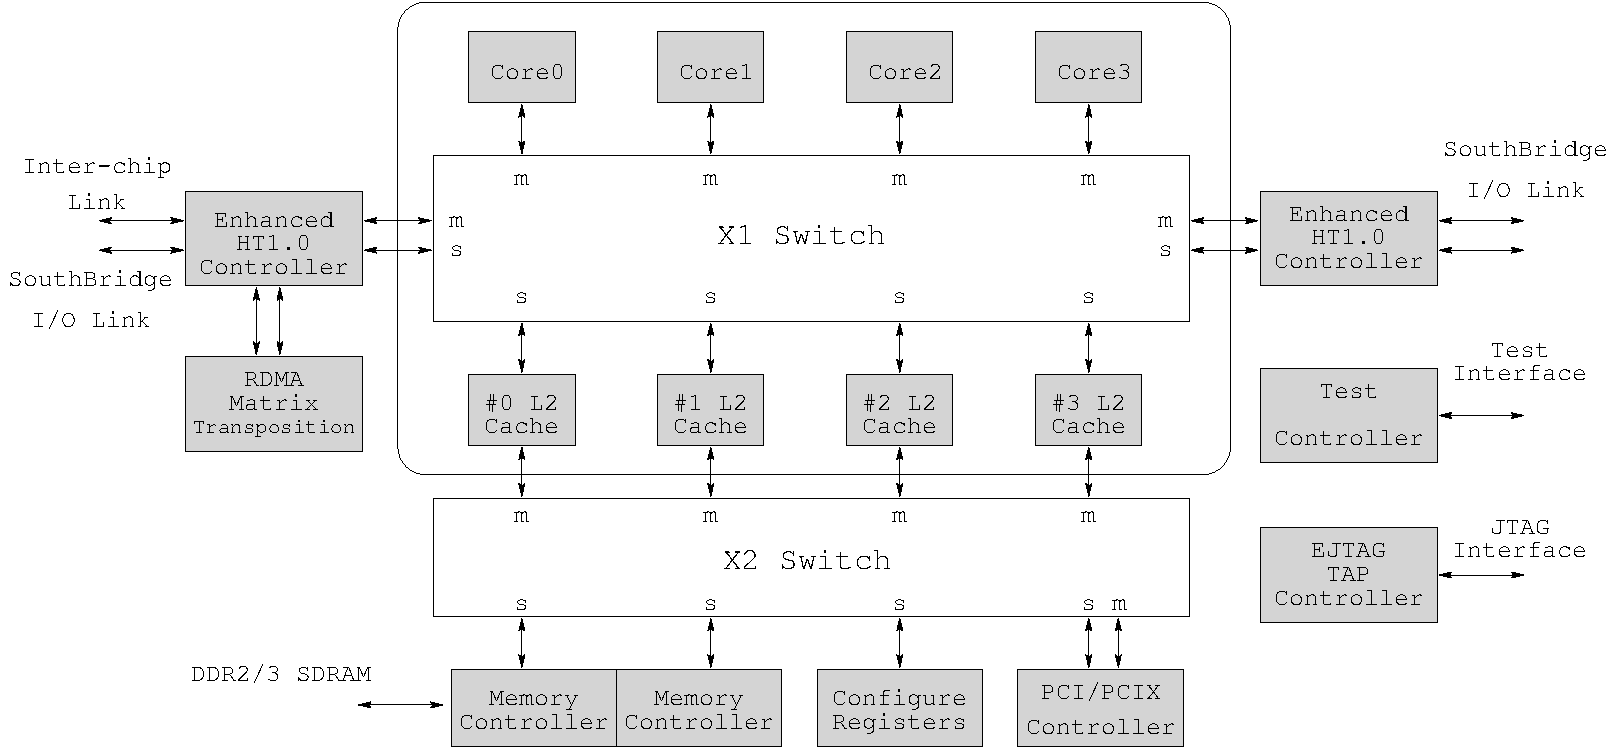
\includegraphics[scale=.5]{gs3a-chip}}
  \caption{龙芯 3A 芯片结构}
  \label{fig:ls3a-structure}
\end{figure}

龙芯 3A 的第一层互连采用了 $6\times6$ 的交叉开关,用于连接四个 GS464 处理器核
(作为主设备) 、四个 二级 Cache 模块(作为从设备) 、以及两个 IO
端口(每个使用一个主端口和一个从端口) 。一级互连开关连接的每个 IO 端口连接一个
16 位的 Hypertransport (HT) 控制器, 每个 16 位的 HT 端口还可以作为两个 8
位的 HT 端口使用。HT 控制器通过一个DMA 控制器和一级互联开关相连,DMA 控制器负责
IO 的 DMA 控制并负责片 间一致性的维护。 龙芯 3A 的 DMA
控制器还可以通过配置实现预取和矩阵转置。 第二级互连采用 5x4 的交叉开关, 连接 4
个 2 级 Cache 模块 (作为主设备) , 两个 DDR2 内存控制器、低速高速 I/O(包括
PCI、LPC、SPI 等)以及芯片内部 的控制寄存器模块。
上述两级互连开关都采用读写分离的数据通道,数据通道宽度为 128 位,工
作在与处理器核相同的频率,用以提供高速的片上数据传输。 

龙芯 3A 采用 65nm 工艺制造, 最高工作主频为 1GHz。 其主要技术特征如下:
\begin{itemize}
	\item 片内集成 4 个 64 位的四发射超标量 GS464 高性能处理器核;
	\item 片内集成 4 MB 的分体共享二级 Cache(由 4 个体模块组成,每个容量为 1MB) ;
	\item 通过目录协议维护多核及 I/O DMA 访问的 Cache 一致性;
	\item 片内集成 2 个 64 位 400MHz 的 DDR2/3 控制器;
	\item 片内集成 2 个 16 位 800MHz 的 HyperTransport 控制器;
	\item 每个 16 位的 HT 端口可以拆分成两个 8 路的 HT 端口使用;
	\item 片内集成 1 个 32 位的 100MHz PCIX/66MHz PCI 接口;
	\item 片内集成 1 个 LPC、2 个 UART、1 个 SPI、16 路 GPIO 接口。
\end{itemize}

\noindent 根据系统组成结构的不同,龙芯 3A 有两种工作模式:
\begin{enumerate}
  \item 单芯片模式: 系统只集成 1 片龙芯 3A, 构成一个对称多处理器系统 (SMP);
  \item 多芯片互连模式: 系统中包含 2 片或 4 片龙芯 3A,通过龙芯 3A 的 HT
    端口进行互连,构成一个非均匀访存多处理器系统(CC-NUMA)。
\end{enumerate}
基于龙芯 3
号可扩展互联架构,4 片四核龙芯 3A 可以通过 HT 端口连接构成 4 芯片 16
核的对称多处理器系统 (SMP) 结构。

\section{Cache 一致性}

龙芯 3A 实现了通过硬件维护
\begin{itemize}
  \item 通过 HT0 互联的处理器之间的 Cache 一致性,即片间 Cache 一致性;
  \item 通过 HT 端口接入的外设之间的 Cache 一致性。
\end{itemize}
注意,龙芯 3A 的硬件不维护通过 PCI 等慢速总线接入到系统中的 I/O 设备的 Cache
一致性。在驱动程序开发时, 对通过 PCI 接入的设备进行 DMA (Direct Memory
Access) 传输时,仍然需要软件进行 Cache 一致性维护。

